As discussed in previous sections, the choice of certain software, protocols, or
techniques such as X509 certificates or PGP web of trust has implications in the
level of horizontality possible for systems built on top of those software,
protocols, or techniques. How, then, can we build a foundation such that
organizations of different horizontality can use the same foundation and arrive
at much differently structured organizations?

In this section we describe Collective Based Access Control, or COLBAC: our
approach to a dynamic horizontality access control system. We begin by
describing its requirements, focusing on the dynamic horizontality that
separates COLBAC from other access control systems. We then define the system
itself. Finally, we discuss the properties and in Section~\ref{sec:limitations}
we discuss the limitations of this system. Though this is, to our knowledge, the
first attempt at defining a collective based access control system with dynamic
and flexible horizontality, it is far from the only potential approach. Section
\ref{sec:future_work} discusses some potential future work to improve upon it.

To our knowledge COLBAC is the first attempt to incorporate democratic processes
into access control. However, democracy is a complex concept, and COLBAC only
incorporates some aspects of democracy. For example, solution is not utilized
at all in COLBAC. For our definition of the \textit{Demos}, we consider all
members of a system using COLBAC do be part of the \textit{Demos} and thus
eligible to vote. Our design of COLBAC also assumes there exists an external
channel for deliberation that is used by all members of the \textit{Demos}, and
that there may exist external channels for other forms of decision-making.
However, every decision made in these external channels that affects the system
must eventually become a vote within COLBAC.

Given these assumptions and the design of COLBAC, we can see that COLBAC allows
for a large variety of different democratic governance schemes. More direct
forms of democracy can be done using Action Tokens, and elective representation
can be done using Delegation Tokens\footnote{These types of Tokens are described
in Section~\ref{sec:Tokentypes}}. The spectrum between full consensus and
majority decision-making is represented through the security parameter $f$ and
the decision of how much participation is required per vote and, therefore, how
difficult it is to create a quorum can be fine-tuned using the security
parameter $m$\footnote{These security parameters are described in Section
\ref{sec:colbacdesign}}.

\subsection{System Requirements}
\label{sec:colbacrequirements}
COLBAC is aimed at addressing a novel requirement in Cybersecurity research:
access control and authorization given an organization with dynamic levels of
horizontal control. Though previous approaches exist for hierarchical access
control (such as MAC, RBAC, etc.), to our knowledge no access control model
exists for organizations of dynamic and flexible horizontality. To realize
this, our solution must be able to be flexible in terms of horizontality. Said
another way, our system must not assume or define a pre-determined threshold for
horizontal control, i.e., it must not assume majority, or super-majority, or
full consensus is the preferred method of democratic participation. Instead,
the threshold must be configured by the collective itself, and must be able to
be changed when necessary. This allows for rapid temporary centralization of the
system to respond to crises, or to perform a task that requires expertise that
few members of the collective contain. However, these moments of centralization
must be quick to expire and easy to override in order to prevent abuse of
centralized power. Said another way, it must always be easier for the collective
to return to more horizontal control than for a centralized entity to maintain
control over the system.

However, it makes no sense to have horizontal or democratic control without
transparency. An individual cannot meaningfully vote or otherwise decide on a
practice, or place confidence in a representative, without understanding what
the action is going to take place, and what actions have been taken in the past.
More, if authority is abused, the collective must be able to notice the abuse,
and remove the powers that allowed the abuse to take place. Thus, we can see
that any horizontal access control system requires transparency. Towards this
end, our system must have a method of logging information about the actions of
individuals and the collective that is immutable and available.

\subsection{System Design}
\label{sec:colbacdesign}
COLBAC presents a solution to access control that relies on the collective.
However, as will be discussed later in this section, not all objects on the
system will need to be collectively controlled or administered. As such, we
define three distinct \textit{spheres} of the system, or areas that require
different approaches to access control. These spheres are the \textbf{Collective
Sphere}, the \textbf{User Spheres}, and the \textbf{Immutable Sphere}.

In order to achieve different degrees of horizontality, there must be a portion
of the system that is controlled not by any individual user of the system, but
by some democratic process of the users of the system. We call this portion of
the system the \textbf{Collective Sphere}, as it contains programs, files, and
other resources only accessed based on collective authorization. In any
horizontal system, the administrative functions of the operating system would
need to exist within this portion of the system to allow for true collective
control. Additionally, all services that the collective offers, or official
sources of collective information, must also exist in this sphere.

However, not everything should be directly managed by the collective. Individual
users may have their own files and programs, which they intend to use only in
ways that do not affect other users of the system or the resources of the
collective\footnote{We can think of these as the home directories of users in
modern Unix-like systems.}. This sphere, called the \textbf{User Sphere},
can use traditional DAC systems like modern Unix-like systems without affecting
the horizontality of the system as a whole.

Finally, to have meaningful control of the system we must have transparency. To
achieve this, a system must have an \textbf{Immutable Sphere}, or a portion of
the file system and programs that cannot be altered once written to, including
by democratic control. This allows for the system to provide append-only logs
that are vital to maintaining collective control, as described later in this
section. Additionally, this section can hold a list of inalienable rights that
each participant in the system has, such as the right to a vote.

When the system is first installed, a \textit{Registration Phase} will occur.
During this phase, at least 3 users will be signed up in the system. These users
will need to supply their public keys, which correspond to offline private keys,
since they will be needed for later interactions with the system. In addition to
supplying their public keys, the users will need to decide on an initial
fraction $f$ and a minimum fraction $m$ that will be used for action and
delegation petitions, as explained later.

After the system is set up, users can interact with objects in the User Sphere
as they would in any other system. However, to interact with any objects in the
Collective Sphere, users would need to follow a specific authorization
procedure consisting of three phases: the \textit{Draft Phase}, the 
\textit{Petition Phase}, and the \textit{Authorization Phase}.

In the Draft Phase, depending on the action the user wishes to perform, they
will write the code or commands that will interact with objects in the
Collective Sphere, or will identify the permissions they will need to accomplish
their task or tasks. At the end of this process, the user will have a draft
Action or Delegation Token, as described later in Sections \ref{sec:Tokentypes}
and \ref{sec:Tokenformat}.

After the user has completed their Token, they move on to the Petition Phase. In
this phase the user sends their draft Token to the reference monitor running on
the system. This reference monitor will then forward the draft Token to all
other members of the system and ask for a vote. The users will then vote one of
the following ways: yes, no, or abstain\footnote{It is important to mention that
this is not the only way of performing democratic participation. However, other
models of democratic participation are left to future work.}. The system will
wait for a pre-configured amount of time before marking all individuals who did not
vote as abstaining.

After all votes are collected or the response period has timed out, the system
enters the authorization phase. During the action phase the reference monitor
counts all of the votes. If the number of votes divided by the total number of
users is greater than or equal to $m$, and the fraction of yes votes to the
total number of votes is greater than or equal to $f$, the petition is
considered successful and the token is returned to the petitioning user. In
addition to taking the action, the system logs the action in log files held in
the immutable sphere. However, if the number of all votes divided by the total
number of users is less than $m$ or if the number of yes votes divided by the
total number of votes is less than $f$, the petition fails, and the attempted
action is logged in the immutable sphere.

\subsection{Types of Tokens}
\label{sec:Tokentypes}
As the previous section demonstrates, the Token is the main form of interacting
with the Collective Sphere. Users who wish to affect the Collective Sphere do
so by creating a Token which is then voted on by the users of the system. In
order to facilitate easy interaction with the COLBAC system, there are multiple
types of Tokens.

The first Token is called the \textbf{Action Token}. This Token allows a single
command, a small script, or a program to be run in the Collective Sphere, and to
enjoy Collective Sphere access. This is the most straightforward type of Token,
since everything the Token will allow to occur is known during the Petition
Phase. However, this type of Token is rigid and inflexible. If there is an error
in the command, or in the code, a user would need to re-enter the Draft Phase,
fix the error, and re-enter the Petition Phase to authorize a new Token. The
more a single Action Token attempts to do, the more likely there will be errors,
causing frustration for both the users drafting the Tokens and the users voting
on them.

To avoid these issues, COLBAC also allows for \textbf{Delegation Tokens}, which
allow the drafting user to act in the Collective Sphere for a given set of time,
and with a given set of restrictions. The procedure is obtaining a Delegation
Token is the same as that for an Action Token. However, the information that
would be put in the Token would be slightly different. The format for Action
Tokens and Delegation Tokens are shown in Section~\ref{sec:Tokenformat}.

Consider the example of the democratically run trade union introduced in Section 
\ref{sec:introduction}. In this example, a new communication committee was put
in power though a slate of democratic elections. However, former individuals who
had access to read the emails that arrived to the collective's inbox did not
allow members of the new committee to read or send emails. If this trade union
had been using COLBAC, after the elections a Delegation Token would have been
drafted to grant the new committee access to both read and send emails. This
Delegation Token would then gone through a Petition Phase, where presumably it
would pass\footnote{This assumption is based off of the results of the
democratic elections that occurred before.}. Thus, the individuals previously in
charge of email would be incapable of denying access to the new committee.

There are some instances in which one needs to respond to emergency situations
as soon as possible, and cannot wait for a slow authorization process by a
potentially large set of users. To accommodate these situations, COLBAC has an
\textbf{Emergency Token}. These Tokens allow users to run short scripts, single
commands, or small programs in the Collective Sphere without immediate
authorization. However, this action is immediately logged and all users are
informed by the Reference Monitor that an Emergency Token was used. In the case
that an Emergency Token was incorrectly used (say, to overwrite the result of
a democratically made decision), a member can create a new Action Token to
undo the actions of the Emergency Token, which will be pushed to a Petition
Phase for democratic decision making. To avoid large-scale misuse of the
Emergency Token, and to avoid Emergency Token Wars\footnote{We define Emergency
Token Wars as instances in which different members in the organization use
Emergency Tokens to undo the actions taken in the name of the collective.},
each member only has a small number of emergency Tokens for a given period of
time. Additionally, there are limits placed on what can be done with Emergency
Tokens.

\subsection{Token Format}
\label{sec:Tokenformat}
\begin{figure}
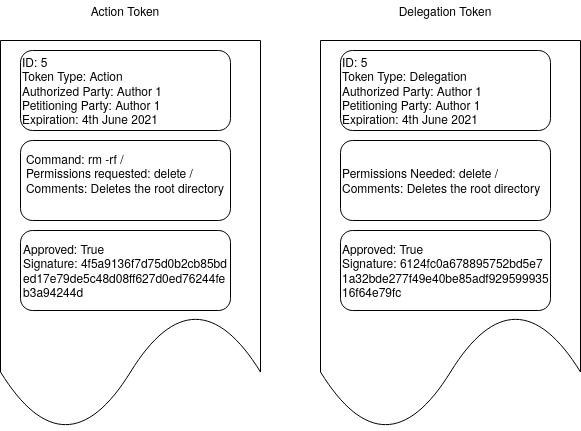
\includegraphics[width=\linewidth]{figs/TokenStructures.png}
\caption{COLBAC Token Structures}
\label{fig:Tokenformatfigure}
\end{figure}
Each Token contains three sections, a header, a body, and a footer. Different
types of Tokens (action Tokens, delegation Tokens, or emergency Tokens) contain
different fields in their body sections. However, the headers and footers of all
Token types contain the same fields. For a graphical representation of the Token
format, please see Figure~\ref{fig:Tokenformatfigure}.

The first portion of a Token is called the header. The header contains the
following fields:
%Header:
\begin{enumerate}
\item \textbf{Nonce/ID}:\\ 
An integer used to both identify the Token and avoid replay attacks.
\item \textbf{Token Type}:\\ 
The type of Token. Can only be Action, Delegation, or Emergency.
\item \textbf{Party(s) Being Authorized}:\\
A single entity or set of entities requesting authorization to perform an action
or set of actions in the Collective Sphere.
\item \textbf{Petitioning Party}:\\
The single entity petitioning for authorization. This user usually also exists
in the list of parties being authorized.
\item \textbf{Token Expiration}:\\
The expiration time of the Token in Unix format.
\end{enumerate}

For Action Tokens or Emergency Tokens, the Token body contains the following
fields:
\begin{enumerate}
\item \textbf{Code to be Run}:\\
The command, script, or program to be run in the Collective Sphere.
\item \textbf{Permissions Requested}:\\
A set of permissions requested to complete the task. These permissions include
negative and positive permissions, of which negative permissions take
precedence. The inclusion of both negative and positive permissions make it
easier for permissions to be specified. For example, if a folder in the
Collective Sphere contains 950 files, and the code running needs read access to
940 of them, it is easier to specify positive read permissions on the whole
folder and negative read permissions on the 10 files, rather than specify 940
positive read permissions and no negative read permissions.
\item \textbf{Comments (optional)}:\\
Comments explaining what the code included in the Token does, and why it is
necessary. This field is similar to messages included in version control systems
like a Git commit message.
\end{enumerate}

For Delegation Tokens, the body contains the following fields:
\begin{enumerate}
\item \textbf{Permissions Needed}:\\
Similar to the set of permissions requested in the Action or Emergency Token
body.
\item \textbf{Comments (optional)}:\\
Similar to the comments section of the Action or Emergency Token body.
\end{enumerate}

As we can see, the Delegation Token body is similar to the Action or Emergency
Token body, except in that it does not specify the code that is running. This
design is ideal for sessions that require troubleshooting, or tasks that may
require back-and-forth between the system and the individual or group performing
the task. However, when using Delegation Tokens it is
more important to ensure that the Permissions Needed section follows the
principle of least privilege. If not, individuals can use the privileges they
gain from the Delegation Token to perform actions that were not originally
intended for their task(s). Though these actions will be logged into the
Immutable sphere, it still requires time and effort of the system users to undo
the actions of an individual who abused the power granted to them through
Delegation Tokens.

Each Token, regardless of type, ends with a footer. The footer simply contains
one field, a field which states if it is approved or denied, along with a
verifiable authentication value that is difficult to predict and easy to verify,
such as an HMAC of the permission Token keyed by a secret value known only to
the Reference Monitor.

\subsection{Formalizing COLBAC}
\label{sec:colbacformal}
In this section we formalize COLBAC, a collective based access control system.
To begin, we define important sets. We then go on to discuss which permissions
are possible in COLBAC, what abbreviations are used in our notation, and what
functions we rely on in our formalization. Finally, we introduce different
algorithms used by the reference monitor in our proposed model. This
formalization serves as a basis for our access control model.
\begin{definition}[Spheres of COLBAC]\label{def:spheres}
In COLBAC, a \textbf{Sphere} is a set which contains both subjects (users,
processes, etc.) and objects (files, etc.).\\
\mbox{}\\
Let $U$ be the User Sphere, $I$ be the Immutable Sphere, and $C$ be the
Collective Sphere. Let $\xi$ be the set of all subjects and objects in the
system. Let $\emptyset$ be the Empty Set. These sets have the following
properties:\\
\mbox{}\\
$U \cup I \cup C = \xi$\\
$U \cap I = \emptyset$\\
$U \cap C = \emptyset$\\
$I \cap C = \emptyset$\\
\hrule \mbox{}\\
\end{definition}

\noindent In addition to the sets above, our access control model also requires
a set of permissions, similar to the sets of permissions used in other access
control systems. These permissions will be used later when the reference monitor
is deciding whether or not to permit an action.

\begin{definition}[Permissions in COLBAC]\label{def:permissions}
$Create$ allows the creation of an object.\\
$Append$ allows a subject to append to the end of an object.\\
$Write$ allows arbitrary rights to an object. \\
$Read$ allows a subject to read from an object.\\
$Delete$ allows a subject to delete an object. \\
$Execute$ allows a subject to run an object as a program.\\
\hrule \mbox{}\\
\end{definition}
%\begin{itemize}

%\noindent Before introducing the main algorithms involved in COLBAC, we first
%need to define a few functions. However, to save space some shorthand is used.
%For the functions to follow, we will use the following short-hand:

%\begin{definition}[Abbreviations Used in COLBAC Functions]
%\begin{itemize}
%Let $u$ be a user of the system.\\
%Let $s$ be the subject attempting access.\\
%Let $o$ be the object or set if objects the user is attempting to access.\\
%Let $p:$ be the set of permissions the user is requesting.\\
%Let $t$ be the type of Token the user is attempting to create.\\
%Let $e$ be the proposed expiration time of the Token.\\
%Let $c$ be the comment attached to a Token, or in the case it doesn't exist,
%let $c$ be $NULL$.\\
%Let $a$ be the action\footnote{command, script or program} the user wants to run
%in the Collective Sphere, or in the case that it doesn't exist, let $a$ be 
%$NULL$.\\
%Let $d$ be the set of delegates the user is proposing, or in the case where it
%doesn't exist, let $d$ be $NULL$.\\
%Let $DAC(s :$ Subject$, o:$ Object$)$ be a Discretionary Access Control
%system.\\
%\hrule \mbox{}\\
%\end{definition}

\noindent The first important function we need to define is the $GetSphere$
function. When passed a subject or object, the $GetSphere$ function will return
the Sphere that the subject or object belongs to. Given the properties mentioned
in Definition~\ref{def:spheres}, we can see that a subject or object will be in
exactly one Sphere, meaning that this function will never return $NULL$ or more
than one value.

\begin{definition}[GetSphere]\label{def:getsphere}
$GetSphere(o:$ Subject or Object$) \rightarrow U$ iff $o \in U$, $C$ iff $o \in 
C$, $I$ iff $o \in I$\\
\hrule \mbox{}\\
\end{definition}

\noindent A very important building block of COLBAC is the \textbf{Token}, which
is a primitive taken from Capability based access control. A Token will allow a
subject which exists in $U$ to perform an action on an object that exists in
$C$. These Tokens can be of type \textbf{action}, denoted by a sub-scripted $a$,
\textbf{delegation}, denoted by a sub-scripted $d$, or \textbf{emergency},
denoted by a sub-scripted $e$. Before authorization, a Token is first created by
a $DraftToken$ function, which calls one of the following three functions
depending on the type of Token the subject wishes to create. In addition, COLBAC
requires a function to get the type of a given Token.
\begin{definition}[Token Functions]\label{def:Tokens}
Let $u$ be a user of the system.\\
Let $o$ be the object or set if objects the user is attempting to access.\\
Let $p$ be the set of permissions the user is requesting.\\
Let $t$ be the type of Token the user is attempting to create.\\
Let $e$ be the proposed expiration time of the Token.\\
Let $c$ be the comment attached to a Token, or in the case it doesn't exist,
let $c$ be $NULL$.\\
Let $a$ be the action\footnote{command, script or program} the user wants to run
in the Collective Sphere, or in the case that it doesn't exist, let $a$ be 
$NULL$.\\
Let $d$ be the set of delegates the user is proposing, or in the case where it
doesn't exist, let $d$ be $NULL$.\\
$DraftToken(u,o,p,e,a,c,t) \rightarrow T$ of type $T_{a}$ or $T_{d}$ or 
$T_{e}$\\
$DraftToken_{a}(u,o,p,e,a,c) \rightarrow T_{a} = (u,o,p,e,a,c)$\\
$DraftToken_{d}(u,o,p,e,d,c) \rightarrow T_{d} = (u,o,p,e,d,c)$\\
$DraftToken_{e}(u,o,p,a,c) \rightarrow T_{e} = (u,o,p,a,c)$\\
$GetTokenType(t:$ Token$) \rightarrow \{$the type of Token $t$ from $Action$,
$Delegation$, or $Emergency$\}
\hrule \mbox{}\\
\end{definition}

\noindent Unlike other capability based access control systems, COLBAC does not
rely on a centralized authority or resource owner in the system to grant
capability Tokens. Instead, when a Token is drafted by the user requesting it,
the Token enters a $Petition$ function, which sends the Token to all other
users\footnote{Here we mean human users of the system, not subjects or user
accounts on the system that don't correspond to humans.} of the system for a
participatory decision-making process on whether or not the Token should be
authorized. This $Petition$ function returns a set of Votes on the Token $T$,
referred to as $V_{T}$, and can only be called on Tokens of type \textit{action}
or \textit{delegation.}

Let's consider again the example of the democratic trade union presented in
Section~\ref{sec:introduction}. As mentioned in Section~\ref{sec:Tokentypes},
in COLBAC this change of power would occur through a Delegation Token. Relating
to the notation in Definition~\ref{def:Tokens}, if \textit{u} were a member of
the committee, $o$ was the set of files, folders, and programs needed to read,
write, and send emails, $p$ was the necessary set of permissions to perform
these actions\footnote{Such as the $Execute$ permission for the email program,
the $Create$ and $Write$ permission for temporary files, the $Read$ permission
for the files the emails are stored in, etc.}, $e$ was the expiration date of
the Token\footnote{Which should be set to the last day of the mandate of the
elected body.}, $d$ was the list of all members of the committee, and $c$ was
any human-readable comment the token drafter deemed necessary. Then, the token
drafter would compute $T_{d} = DraftToken_{d}(u,o,p,e,d,c)$, and run
$Petition(T)$ as follows.

\begin{definition}[Petition Function]\label{def:petition}
Let $T$ be a Token created through $DraftToken$.\\
$Petition(T) \rightarrow \{$set of votes $V_{T}$ on authorizing $T$ iff $T$ is
of type $T_{a}$ or $T_{d}$, else $NULL$\}.\\
\hrule \mbox{}\\
\end{definition}

\noindent This Petition Phase would collect votes from all of the members on the
system. The returned set of votes, $V$, can then be split into more useful
sets, such as the set of votes that affirm the authorization of $T$,
$V_{(T, Yes)}$, the set of votes that negate the authorization of $T$,
$V_{(T, No)}$, and the set of abstentions, $V_{(T, Blank)}$. After votes are
sorted into their respective sets, the process of authorizing the votes comes
down to a simple task of comparing the number of votes to fractions of voters
initially defined at system registration. Said another way, a function called
$AuthorizeToken$ will count the votes and compare the results to two security
parameters, $f$, or the fraction of yes votes required to authorize a Token, and
$m$, the fraction of voters required to participate in order for a vote to be
considered. These two security parameters are chosen at the initialization of
the system, and can be changed by a successful action Token\footnote{These
parameters cannot be changed by a delegate or by an emergency Token. This is
discussed more in Section \ref{sec:colbacproperties}.}. If the vote is
successful, the Token is then authorized by the addition of a signature field
that is difficult to predict or replicate, but easy for the reference monitor to
later verify. One example of this is a keyed HMAC.
%\begin{definition}[Sets of Votes]\label{def:votes}
%$V_{(T, Yes)} = \{v \in V$ s.t. $v = True\}$\\
%$V_{(T, No)} = \{v \in V$ s.t. $v = False\}$\\
%$V_{(T, Blank)} = \{v \in V$ s.t. $v = NULL\}$\\
%\hrule\mbox{}\\
%\end{definition}

\begin{definition}[Authorization in COLBAC]
Let $V$ be the set of all votes on token T.\\
Let $V_{(T, Yes)} = \{v \in V$ s.t. $v = True\}$\\
Let $V_{(T, No)} = \{v \in V$ s.t. $v = False\}$\\
Let $V_{(T, Blank)} = \{v \in V$ s.t. $v = NULL\}$\\
$AuthorizeToken(T,V_{T}) \rightarrow True$ iff $\frac{|V_{(T, Yes)}|}{|V|} > f
\wedge \\ \frac{|V_{(T,Yes)} \cup V_{(T, No)}|}{|V|} \ge m$, else $False$\\
\hrule\mbox{}\\
\end{definition}

The process of determining authorization in COLBAC occurs in one or two phases,
depending on which Sphere contains the object the subject wants to access.
If the object is in the User Sphere, the reference monitor simply performs a
traditional DAC check, like one would see on a typical Unix-like operating
system.

If the object is in the Collective Sphere, the subject is expected to
provide a previously authorized Token or draft a new Token for the reference
monitor. If the subject provides a previously authorized Token, the validity of
that Token is checked, and if it is valid, the action is taken. If the subject
does not have a valid Token, they instead provide a draft Token. The reference
monitor then takes this draft Token and enters the Petition phase, where all
users of the system are given the opportunity to vote on the Token. If the
petition succeeds, the Token is authorized and returned to the subject. If the
petition fails, the Token is not returned. In either case, the submission of the
Token to the reference monitor is logged in the Immutable Sphere. In the example
provided in Section~\ref{sec:introduction}, all of the data required to access
the collective email exists in the Collective Sphere.

If the object the subject is trying to access is in the Immutable Sphere, the
reference monitor performs a very simple access control check. If the type of
access on the resource in the Immutable Sphere is a $read$ operation, it always
succeeds. This is to provide transparency on the different operations that are
attempted in the Collective Sphere, since the Immutable Sphere mainly contains
logs of what was done in the Collective Sphere. If the type of access on the
resource in the Immutable Sphere is a $write$ operation, it always fails, since
$write$ operations can arbitrarily write to any portion of a file. Likewise,
$delete$ operations and $execute$ operations always fail. If the operation is a
$create$ or $append$ operation, the reference monitor must check that the
subject has a valid Token to do so. If not, they may not perform the action.
The reference monitor, however, may always append or create in the Immutable
Sphere.

An algorithmic representation of these access control decisions are included in
Algorithm~\ref{alg:main}. To continue with our example from Section
\ref{sec:introduction}, imagine that a member of the committee wants to read an
email in the Collective Sphere. We can see that $GetSphere(o)$ would return $C$,
since the email program exists in the Collective Sphere. Thus, the block of code
from lines 14 to 20 would be executed, and the Token would be checked. Assuming
that the previous vote on the Petition Phase for the Delegation Token has
passed, line 14 would return the non-NULL Delegation Token that $u$ has as a
member of the elected committee. Then, since the action that they wish to
perform (read an email) is covered by the permissions of the Delegation Token
$T$, the action will be logged on line 17 and then performed on line 18.
However, if $u$ were not a member of the committee, then the $GetToken$ function
would return NULL, or would return Tokens that do not have the relevant
permissions. As such, lines 22 -- 32 or line 19 would be executed, respectively.

\begin{algorithm}
\caption{The main decision making process of COLBAC}
\label{alg:main}
\begin{algorithmic}[1]
\State Let $u$ be a user of the system.
\State Let $s$ be the subject attempting access.
\State Let $o$ be the object or set if objects the user is attempting to access.
\State Let $p$ be the set of permissions the user is requesting.
\State Let $t$ be the type of Token the user is attempting to create.
\State Let $e$ be the proposed expiration time of the Token.
\State Let $c$ be the comment attached to a Token, or in the case it doesn't exist,
let $c$ be $NULL$.
\State Let $a$ be the action the user wants to run in the Collective Sphere, or in the
case that it doesn't exist, let $a$ be $NULL$.
\State Let $d$ be the set of delegates the user is proposing, or in the case where it
doesn't exist, let $d$ be $NULL$.
\State Let $DAC(s :$ Subject$, o:$ Object$)$ be a Discretionary Access Control
system.
\If{$GetSphere(o)=U$}
    \State Return $DAC(s,o)$
\ElsIf{$GetSphere(o)=C$}
    \State $T = GetToken(u)$
    \If{$T \ne NULL$}
        \If{IsValid($C, T, a$)}
            \State LogAction($a, u$)
            \State PerformAction($a$)
        \Else
            \State LogFailedAction($a, u$)
        \EndIf
    \Else
        \State $T = DraftToken(u,o,p,t,e,c,a,d)$
        \If{$GetTokenType(T) \in (T_{a}, T_{d})$}
            \State $V_{T} = Petition(T)$
            \State $V_{(T, Yes)} = \{v \in V$ s.t. $v = True\}.$
            \State $V_{(T, No)} = \{v \in V$ s.t. $v = False\}.$
            \State $V_{(T, Blank)} = \{v \in V$ s.t. $v = NULL\}$.
            \If{$AuthorizeToken(T, V_{(T, Yes)}, V_{(T, No)}, V_{(T, Blank)},f, m)$}
                \State LogSuccess($T$)
                \State Return $T$
            \Else
                \State LogFailure($T$)
            \EndIf
        \EndIf
    \EndIf
\Else
    \State $T = GetToken(u)$
    \If{IsValid($I, T, a$)}
        \State LogAction($a, u$)
        \State PerformAction($a$)
    \Else
        \State LogFailedAction($a, u$)
    \EndIf
\EndIf
\end{algorithmic}
\end{algorithm}

Perhaps the most important part of this logic lies in the IsValid function. This
function must ensure that the Token itself has been issued by the reference
monitor, that the Token has not expired, and that the permissions of the actions
that the Token grants are consistent with what the action is attempting to do.
In the case that one of these three conditions is not true, the reference
monitor must not perform an action. We present the logic of the IsValid function
in Algorithm~\ref{alg:isvalid}.

To understand this Algorithm we still need to introduce one more function
definition. In order to be able to decide whether or not a given action should
be allowed, the reference monitor must be able to see what permissions the
action the subject is supplying requires. Thus, we introduce the
GetRequiredPermissions function as follows. This function works on the level of
commands, instead of actions, to allow for granular identification of which
portion of the action is causing issues (if indeed the action is longer than one
command).

\begin{definition}
GetRequiredPermissions$(c:$ Command$) \rightarrow$ \{the set of permissions,
$p'$ needed to complete the proposed command.\}\\
PermissionType$(p:$ Permission$) \rightarrow $ \{the type of access the
permission is requesting among the permissions listed in Definition
\ref{def:permissions}\}\\
\hrule\mbox{}\\
\end{definition}

\begin{algorithm}
\caption{The IsValid function of COLBAC.}
\label{alg:isvalid}
\begin{algorithmic}[1]
\Procedure{IsValid}{$S$: Sphere, $T$: Token, $a$: Action}
\State Let $C$ be the Collective Sphere.
\State Let $I$ be the Immutable Sphere.
\If{$S = C$}
    \If{$GetTokenType(T) \neq T_{e}$}
        \For{$c \in a$} \Comment{For each command in the action}
            \State $p =$ GetRequiredPermissions$(c)$
            \If{$p \notin T.p$}
                \State Return $False$
            \EndIf
        \EndFor
        \State Return $True$
    \Else
        \State $p =$ GetRequiredPermissions$(c)$
        \If{CheckEmergencyPermissions($p$) $\neq True$}
            \State Return $False$
        \EndIf
        \State Return $True$
    \EndIf
\ElsIf{$S = I$}
    \For{$c \in a$} \Comment{For each command in the action}
        \State $p$ = GetRequiredPermissions$(c)$
        \If{PermissionType($p$) $\in (write, delete, execute)$}
            \State Return $False$
        \ElsIf{PermissionType($p$) $\in (create, append)$}
            \If{$p \notin T.p$}
                \State Return $False$
            \EndIf
            \State Return $True$
        \Else \Comment{The permission is read}
            \State Return $True$
        \EndIf
    \EndFor
\EndIf
\EndProcedure
\end{algorithmic}
\end{algorithm}

In this paper we leave CheckEmergencyPermissions as yet undefined, but discuss
some possibilities for this function in Section~\ref{sec:colbacproperties}.

\subsection{Properties of COLBAC}
\label{sec:colbacproperties}
In Section~\ref{sec:colbacdesign} we introduced the design of COLBAC, an access
control system meant to serve as a primitive that can be used to achieve a more
horizontal form of security. In Section~\ref{sec:colbacformal} we presented a
more formal definition of the system, filling in some of the details of how the
system worked.

As stated in Section~\ref{sec:colbacrequirements}, the goals of the system
design were to provide flexible and dynamic horizontality, and to provide
transparency such that individuals participating in the system could reasonably
participate in the decision-making process. Through the design of COLBAC we have
created an access control system that meets these goals. We achieve flexible and
dynamic horizontality in our design through the modification of our two security
parameters, $f$ and $m$. We achieve transparency through the use of the
Immutable Sphere, and the logging that our reference monitor does during its
operation (as described in Algorithm~\ref{alg:main}.

Though our design does provide for flexible and dynamic horizontality, it does
not allow for every level of horizontality. For example, in our design a
strictly-hierarchical approach is not possible: even if $f$ is set to
$\frac{1}{n}$, where $n$ is the number of users, that simply means that one
person needs to vote in favor to authorize an action, but it does not say
\textit{which} individual has that power, meaning that any single vote from any
user is capable of authorizing an action. This is far from a dictatorial
structure, in which all power is fixed in the hands of one individual or a small set of
individuals.

This design does allow for many different expressions of horizontal structures,
however. For example, because of the existence of delegation Tokens which expire,
our design allows for an authorization structure that reflects those of
representative democracies, where elected individuals preside over certain
responsibilities in the system. However, if the collective does not approve of
how the elected individual is performing their duties, our solution allows for
users to call for a democratic vote that invalidates the Token of the delegate,
thus forcing a new delegate to be chosen, or bringing the responsibility back
into the collective.

More, our system allows for action Tokens to modify the values of $f$ and $m$,
thus making it possible for an organization to adjust how many individuals in
the collective must agree on authorizing a Token in order for the Token to be
authorized. This allows the organization to decide if they want to work with
a full consensus based approach, a super majority approach, a majority approach,
or something else entirely. A consequence of this system is that it is easier to
require \textbf{more} consensus than it is to require \textbf{less} consensus.
This property is obvious when one realizes that if an organization calls a vote
to switch from $f$ to $f'$ where $f > f'$, that action token still needs $f$
votes, the larger number, to become authorized. However, if the organization
wants to require \textbf{more} consensus, in other words a user petitions a
token to change from $f$ to $f'$ where $f < f'$, then that vote requires $f$
votes, the smaller number of the two, to be authorized. A similar claim can be
made about the amount of interaction required, which would be affected by
changing the security parameter $m$.

Another interesting property of this system is that it contains in it the
inalienable right to vote. Whenever a vote is called, the reference monitor does
not send it to a small set of individuals who are marked as having a right to
vote. Instead, it sends it to all individuals who are a part of the system.
Thus, in the COLBAC system the right to vote is inalienable as long as one
remains part of the system. Likewise, because the reference monitor grants all
read access to any object in the Immutable Sphere and disallows any deletions or
arbitrary writes in the Immutable Sphere, transparency of the system is
guaranteed so long as the reference monitor behaves according to the system
design.

However, in order to avoid the equivalent of a coup d'\'etat on the system, we
must set some limitations of what certain tokens can do. For example, if an 
individual user of the system wishes to perform a coup d'\'etat, one approach
would be to use an emergency token to set $f$ and $m$ to $\frac{1}{n}$ where $n$
is the number of users in the system, then create and authorize action tokens to
remove users from the system until only user accounts that are loyal to that
user remain. To avoid this, there must be limitations on what emergency Tokens
and delegation tokens can do. For this case specifically, emergency and
delegation Tokens must not be able to alter the values of $f$ and $m$. Similarly
there must be a limitation on the number of emergency tokens an individual has,
and individuals with access to delegation tokens must not be able to remove many
members. It is likely that even more restrictions are required to maintain the
safety of the system, but we leave the identification of those limitations, and
further analysis of the properties of COLBAC, to future work.

%\subsection{Limitations of COLBAC}
%\label{sec:colbaclimitations}
%Like all systems, COLBAC is not perfect, and suffers from limitations. Perhaps
%one of the most obvious limitations of COLBAC is its usability and user
%experience. Creating a horizontal access control system with democratic
%participation requires the system to interact with its users much more than a
%traditional operating system. Users will be expected to vote on many Tokens in
%the Petition Phase, and this may cause fatigue in some users. Additionally, 
%having horizontal technological solutions relies on the digital literacy of the
%users: users who know how to audit the commands sent in the petition phase have
%a deeper understanding of the potential effects of their vote. However, these
%problems may be solved through interface design, and through iterative
%development of the access control system.
%
%Additionally, COLBAC has a limitation regarding \textit{which} democratic governance structures
%it can represent. For example, a purely elected representative structure without
%referendums is impossible to create using COLBAC, since the right to petition
%a Token is inalienable in COLBAC. While this may be seen as a positive for many
%horizontally-run organizations, some may also view it as a negative. Finally,
%currently COLBAC does not allow for different values of $f$ and $m$ per file.
%Future research may be needed to determine how this would affect the properties
%of COLBAC, and if it may introduce new attacks.
%
%More, COLBAC focuses only on voting, with strictly set options of yes, no, and
%abstention. Future work should look into more forms of democratic participation,
%including but not limited to random sampling, run-off voting (instant, and
%round based), and more. Another potentially useful feature could be the concept
%of an amendment, or an ability to introduce a change to a petition such as
%removing a permission, or fixing a line of code in the action.
